\documentclass[11pt,british,faculty=ea,layout=titlefont,underline=false,titleUppercase=true,titleUnderline=true,hidelinks]{ugent2016-report}

\usepackage[a4paper, total={6in, 10in}]{geometry}
\usepackage[hidelinks]{hyperref}

\usepackage{graphicx}
\graphicspath{./images/}
\usepackage{caption}
\usepackage{subcaption}

\usepackage[
	backend=biber,
	style=ieee,
	sorting=none
]{biblatex}
\addbibresource{library.bib}

\title{Network and Computer Security}
\subtitle{Summary}
\academicyear{2020-2021}
\author{Lorenzo De Bie}  

\begin{document}
\maketitle
\tableofcontents

\chapter{Introduction} \label{cha:introduction}
\section{Security in the media} \label{sec:security-in-the-media}
	\begin{itemize}
		\item Security <=> User friendly: work of security personel goes unnoticed when everything is good, but they get blamed when things go wrong.
		\item Users remains a security risk:
			\begin{itemize}
				\item Due to lack of knowledge: \citetitle{Rodriguez2014} \cite{Rodriguez2014}
				\item Due to incompetence
				\item Information can stell be shared non-digitally
			\end{itemize}
		\item Nobody is safe: \citetitle{Eeckhaut2014} \cite{Eeckhaut2014}
		\item Privacy vs Security: sacrificing privacy so data can be used for security.
			\begin{itemize}
				\item \citetitle{Derix2013} \cite{Derix2013}
				\item \citetitle{Follorou2013} \cite{Follorou2013}
			\end{itemize}
		\item Check yourself using \url{https://haveibeenpwned.com/}
		\item Privacy vs Health: tracing apps in times of COVID-19
		\item Journalists aren't alwasy exactly IT experts \rightarrow remain a critic, remain sceptic
		\item Future trends: blockchains
			\begin{itemize}
				\item mainly used for data integrity through \textbf{public ledgers}
				\item Used to log activity.
					\begin{itemize}
						\item Detect malicious operations, hackers, foreign surveillance, database modifications
						\item Equally important as access restrictions
					\end{itemize}
			\end{itemize}
		\item Future trends: cyber warface
		\begin{itemize}
			\item Nation wide actions to cause damage or disruption. Can include physical impact and/or harm to human persons
			\item Interesting targets: traffic lights, electricity systems, water filtration, power plants
			\item Stuxnet:
				\begin{itemize}
					\item Worm that targeted Iranian nuclear facilities, damaging centrifuges and other hardware
					\item Most likely an American-Israeli cyberweapon
				\end{itemize}
			\item Petya: ransomware or state attack?
				\begin{itemize}
					\item Focused strongly on Ukraine systems
					\item Made very little money
					\item Either very bugge, or very damaging by purpose: permanent removal of files, nuclear power plants, ministries, metros and banks offline, possible link with assassination of Maksym Shapoval
				\end{itemize}
			\item Future trends: IoT: \citetitle{Ford2013} \cite{Ford2013}
		\end{itemize} 
	\end{itemize}
% end section Security in the media

\section{Example Incidents} \label{sec:example-incidents}
	\begin{itemize}
		\item Ashley Madison (2015)
		\item DNC email leak (2016)
		\item Mirai (2016)
		\item Twitter hack (2020)
	\end{itemize}
% end section Example Incidents

\section{Why do we need security? Why Information Security?} \label{sec:why-do-we-need-security}
	\begin{itemize}
		\item Counterpart of securing material objects
			\begin{itemize}
				\item Material object have some \textbf{value}
				\item Can be stolen or damaged
				\item Cost for security/protection takes into account value and risk of theft/damage
			\end{itemize}
		\item Risk of threats against information security is \textbf{much} greater
		\item Value of information sometimes hard to assess, best estimated by damage caused. Losses cannot be undone
		\item Threats against information include:
			\begin{itemize}
				\item \textbf{Loss} of information
				\item \textbf{Forged} information
				\item \textbf{Unauthorised release} of information
				\item \textbf{Repudiation} of information
			\end{itemize}
		\item Value of information systems hard to asses. Systems used to enable service \rightarrow damage when service unavailable or unreliable
		\item Threats against information systems include:
			\begin{itemize}
				\item \textbf{Unavailability}/disruption of service
				\item \textbf{Unauthorised acces} to service
				\item Threats against exchanged information
			\end{itemize}
		\item Security measures for information systems:
		\begin{itemize}
			\item \textbf{Information Security}: encryption, virus scanners, firewalls\dots
			\item Carry some cost (installation, maintenance, computation time)
			\item dependent on risk and potential damage
		\end{itemize}
	\end{itemize}
% end sec:why-do-we-need-security

\chapter{Basic Concepts} \label{cha:basic-concepts}
	\section{A security model} \label{sec:a-security⁻model}
        \begin{figure}[h]
            \centering
			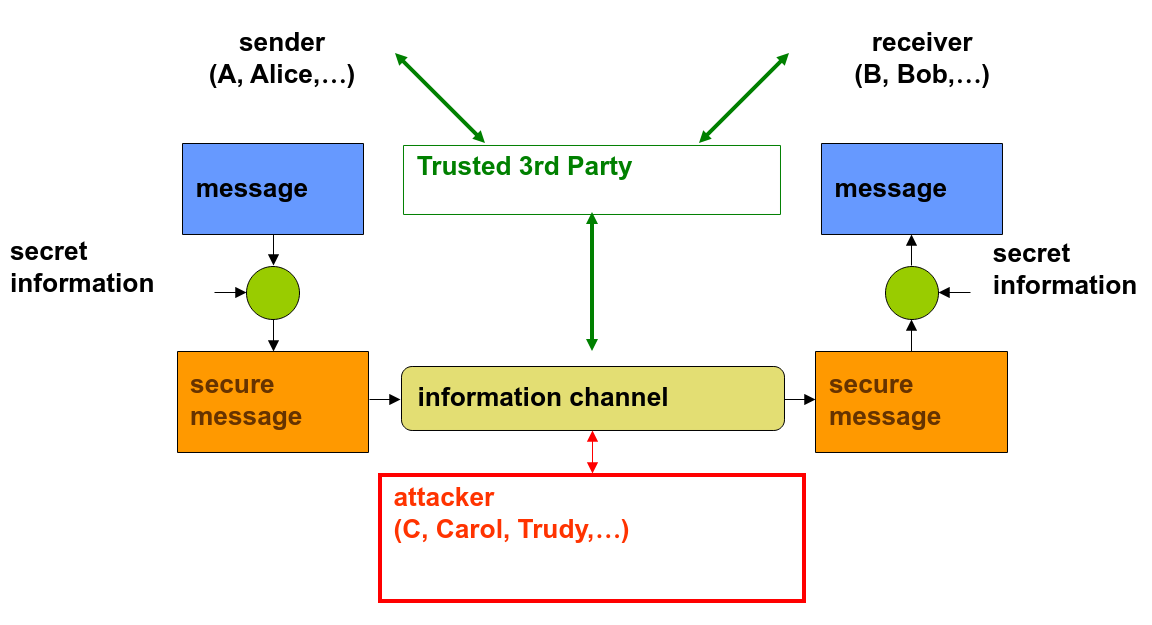
\includegraphics[width=0.6\textwidth]{images/network-security-model.png}    
		\end{figure}
	% end sec:a-security⁻model

    \section{Security Goals} \label{sec:security-goals}
        Possible exam question: \textbf{Which security goals does this protocol fullfill?}
		\subsection{Confidentiality} \label{sub:confidentiality}
            \begin{itemize}
                \item Data can only be read by those who are allowed to read the data
                \item Applications:
                \begin{itemize}
                    \item Communicating confidential data between branches of a corporation
                    \item Passwords
                    \item Storage of health data
                \end{itemize}
            \end{itemize}
            \begin{figure}[h]
                \centering
                \begin{subfigure}{.40\textwidth}
                    \centering
                    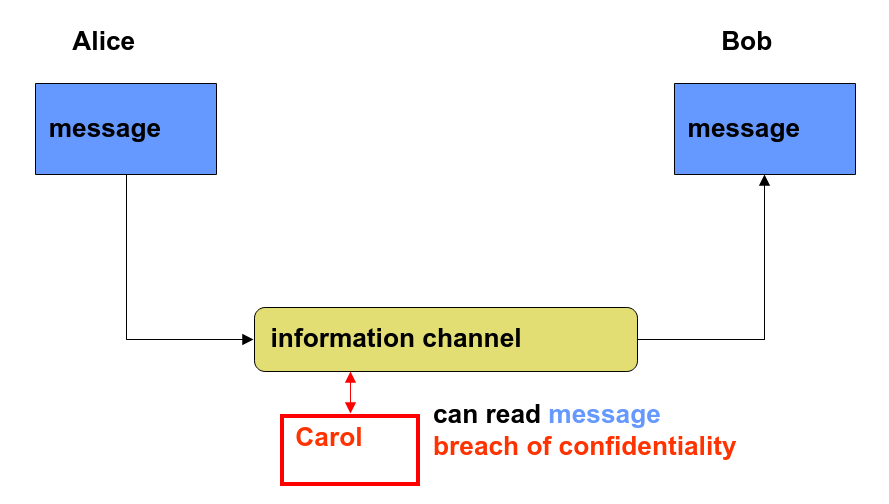
\includegraphics[width=\linewidth]{images/data-confidentiality-threat.png}
                    \caption{Passive attack by Carol: \textbf{eavesdropping} upon information channel}
                    \label{fig:eavesdropping}
                \end{subfigure}
                \begin{subfigure}{.50\textwidth}
                    \centering
                    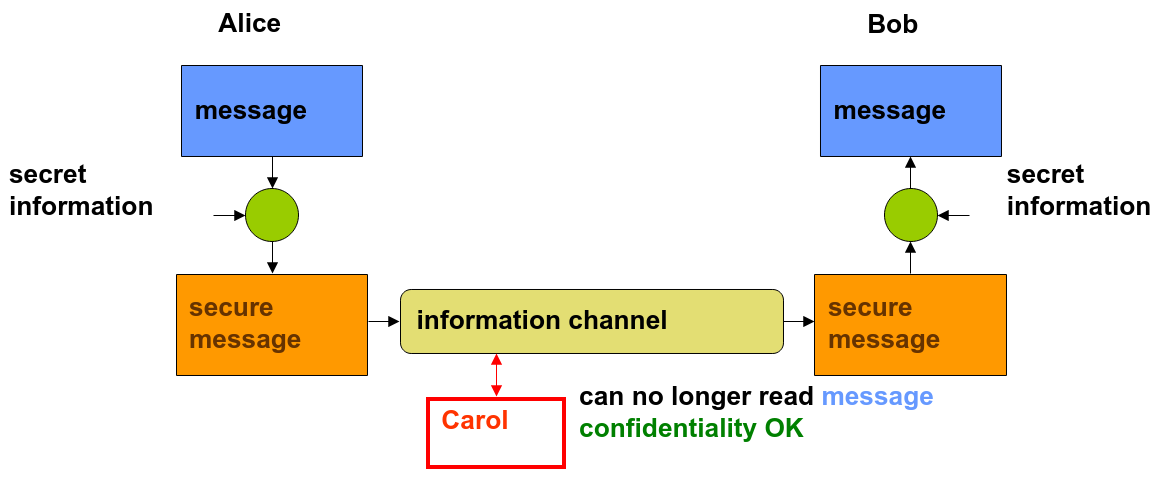
\includegraphics[width=\linewidth]{images/data-confidentiality-solution.png}
                    \caption{Solution to eavesdropping}
                    \label{fig:eavesdropping-solution}
                \end{subfigure}
            \end{figure}
            
            \subsubsection{Traffic-flow confidentiality} \label{subsub:traffic-flow-confidentiality}
                \begin{itemize}
                    \item Keeping secret who's communicating with whom
                    \item Much harder to achieve than data confidentiality
                    \item In \figurename{} \ref{fig:eavesdropping-solution} data confidentiality is OK, traffic-flow confidentiality is NOT OK: Carol can still see that Alice is communicating with Bob
                \end{itemize}
            % end subsub:traffic-flow-confidentiality

            \subsubsection{Confidentiality vs Privacy} \label{subsub:confidentiality-vs-privacy}
                Privacy is having the right to choose what information you give away.
                It is a fundamental right, legally protected since long.
                Not every confidentiality requirement involves privacy: intellectual property in a business requires confidentiality, no privacy.
            % end subsub:confidentiality-vs-privacy
		% end sub:confidentiality

        \subsection{Authentication} \label{sub:authentication}
            Authentication is related to \textbf{identification}: it is the \textit{electronic world} equivalent. \textit{Is the person at the other end of the communication who he claims he is?}

            Guaranteeing teh authenticity of a communication is based on:
            \begin{itemize}
                \item \textbf{Entity} authentication: distinguish each entity from another based on collection of data. Each entity has a unique identity.
                \item \textbf{Attribute} authentication. Attribute = characteristic of an entity. Entities are often authenicated through authentication of some of its attributes. Do the communicating parties exhibit the characteristics they claim to have?
                \item \textbf{Data-origin} authentication: does the data indeed originate from the specified source? Important to evaluate wether data is reliable (\textbf{Data Integrity} see \ref{sub:data-integrity}). Different from entity authentication: \textbf{no interaction with data source}.
            \end{itemize}
            \begin{figure}[h]
                \centering
                \begin{subfigure}{.40\textwidth}
                    \centering
                    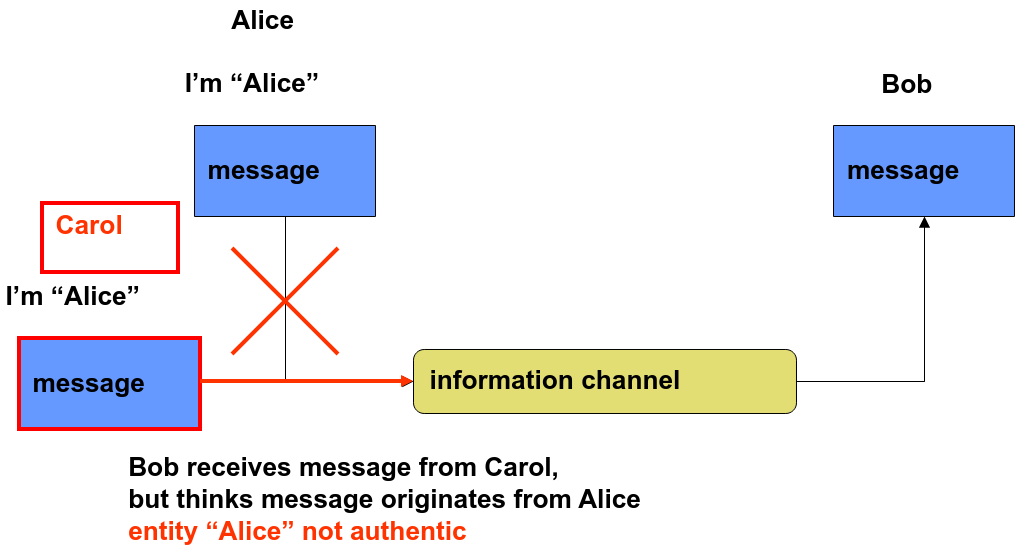
\includegraphics[width=\linewidth]{images/authentication-threat.png}
                    \caption{Threat}
                    \label{fig:authentication-threat}
                \end{subfigure}
                \begin{subfigure}{.50\textwidth}
                    \centering
                    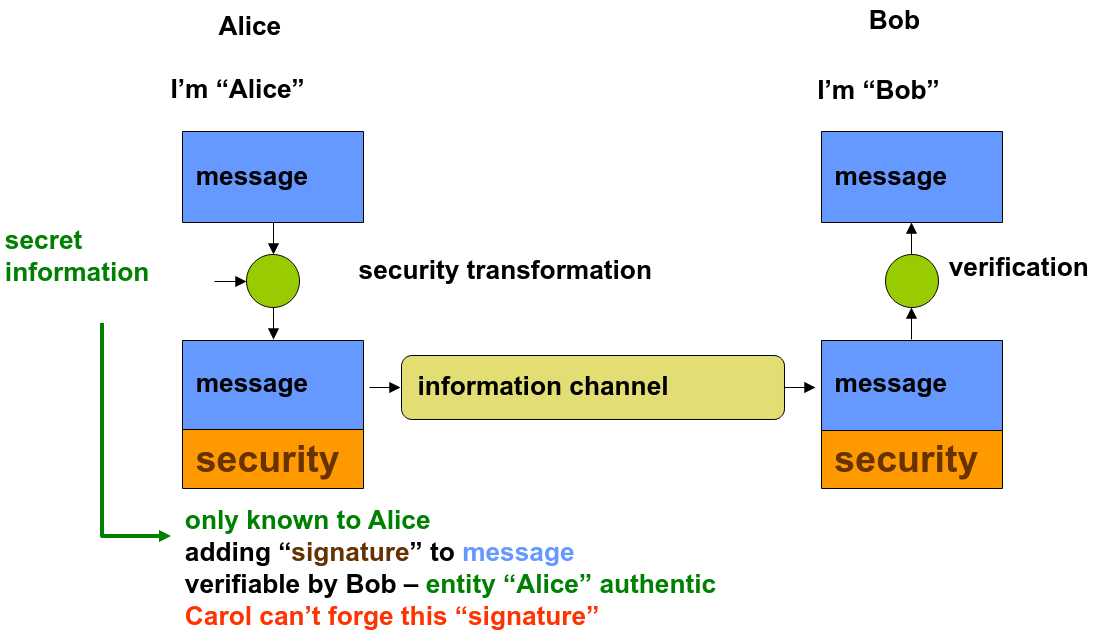
\includegraphics[width=\linewidth]{images/authentication-threat-solution.png}
                    \caption{Solution}
                    \label{fig:authentication-threat-solution}
                \end{subfigure}
            \end{figure}
		% end sub:authentication

        \subsection{Access Control/authorization} \label{sub:access-control-authorization}
            \begin{itemize}
                \item Determines which user may access which resource (data, computation time, etc.)
                \item Requires \textbf{authentication of the entity} requesting access to these resources
                \begin{itemize}
                    \item System determines to what extent entity may access those resources
                    \item Access rights may \textbf{depend on entity itself or its attributes}
                \end{itemize}
            \end{itemize}

            \subsubsection{Illustration 1: access control in OS} \label{subsub:access-control-in-os}
                \begin{itemize}
                    \item Authentication through login and password
                    \item Access control determined for this user (entity)
                        \begin{itemize}
                            \item Full access to own files
                            \item Limited acces to some other files
                            \item No acces to other files
                        \end{itemize}
                    \item Access rights different from user to user
                \end{itemize}
            % end subsub:access-control-in-os
            
            \subsubsection{Illustration 2: access control to medical database} \label{subsub:access-control-to-medical-database}
                \begin{itemize}
                    \item Different rights for different types of Users
                    \item Requires authentication based on specific \textbf{attributes}
                    \item Access rights depend on attributes of the user
                    \item Access rights different from user type to user type (\textbf{roles})
                \end{itemize}
            % end subsub:access-control-to-medical-database

		% end sub:access-control-authorization

		\subsection{Data integrity} \label{sub:data-integrity}
		%end sub:data-integrity

		\subsection{Non-repudiation} \label{sub:non-repudiation}
		% end sub:non-repudiation

		\subsection{Availability} \label{sub:availability}
		% end sub:availability

	% end sec:security-goals

	\section{Security Threats} \label{sec:security-threats}
	% end sec:security-threats

% end cha:basic-concepts

\printbibliography

\end{document}